%% This is an example first chapter.  You should put chapter/appendix that you
%% write into a separate file, and add a line \include{yourfilename} to
%% main.tex, where `yourfilename.tex' is the name of the chapter/appendix file.
%% You can process specific files by typing their names in at the 
%% \files=
%% prompt when you run the file main.tex through LaTeX.

\singlespacing{

\chapter{Related Work}


The following sections outline current research into digital assembly across scales, CAD/simulation packages which occupy a similar space to what I propose, and a detailed description of my proposed work and schedule.

%An active area of synthetic biology explores the possibility of creating a viable cell from scratch based on knowledge about the core systems required for metabolism, cell maintainance, and self replication\cite{Forster2006}.  To date, efforts at creating this "minimal cell" have only been successful using a top down approach - starting with an organism with a minimal genome and reducing its genes further\cite{Glass2006}\cite{Gibson2010}.

\section{Digital Assembly}

Digital assembly is an emerging multimaterial fabrication technique where a finite set of part types are (often reversibly) joined on a regular lattice to for larger structures.  By patterning parts with different material properties across an assembly, programmable function behavior is achieved.  The assembly process is orchestrated by one or many robotic assemblers or a programmable self assembly mechanism.  Self alignment features on the parts and their regular spacing help to minimize the complexity of a robotic assembler, and maintain global metrology through local interactions.

\subsection{Macro Assembly}

Cheung showed that carbon fiber composite parts can be reversibly assembled to form ultralight materials \cite{Cheung2013}.  This work demonstrated programmable flexibility in the structures by pattering rigid and flexural elements across an assembly.  Additional research into digital assembly of structural elements is ongoing at CBA, including modeling of the parts and assemblies using finite element analysis\cite{Calisch2014} and designing new part geometries and robotic assemblers\cite{Carney2015}.

\subsection{Micro Assembly}

%\begin{figure}
%  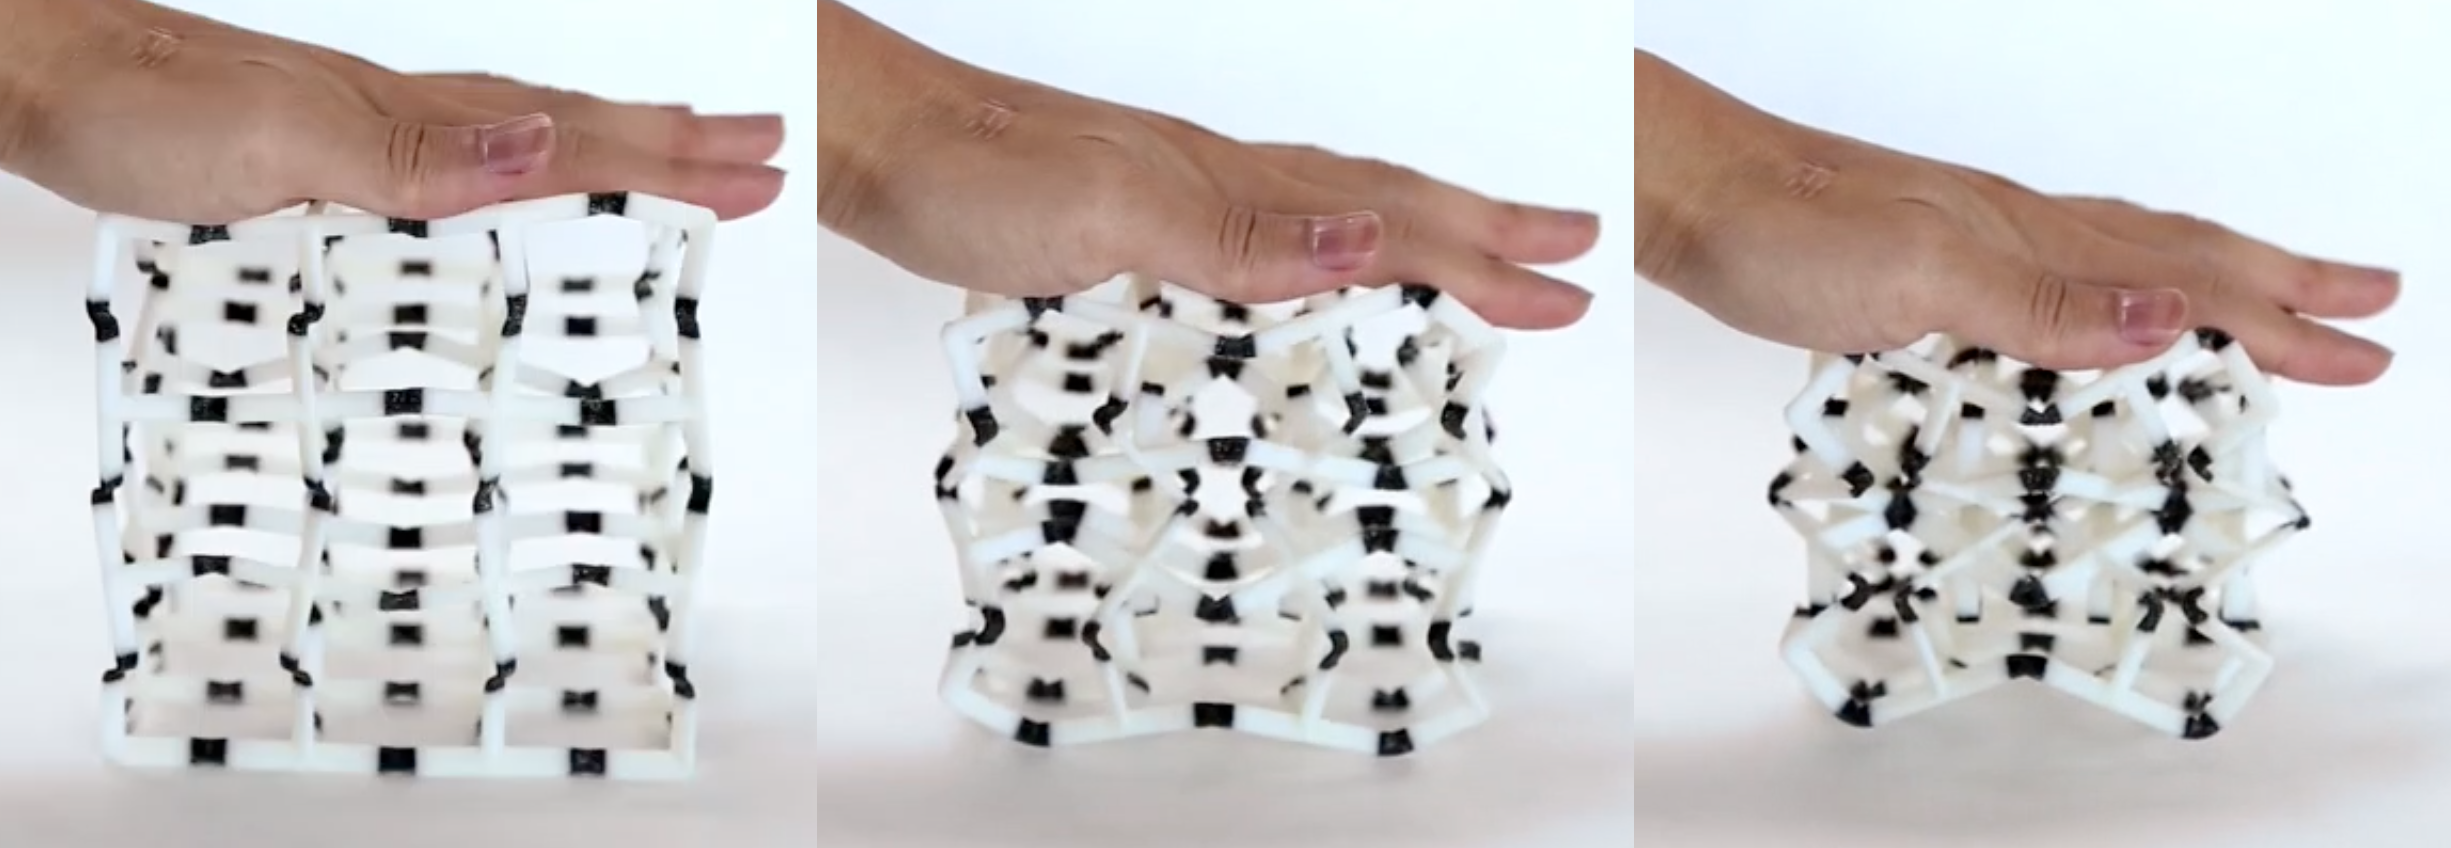
\includegraphics[width=\linewidth]{objetMultimaterial.png}
%  \caption{Mechanical properties programmed by material deposition in Objet 3D print.}
%  \label{fig: objetMultimaterial}
%\end{figure}

Langford demonstrated how conducting, insulating, and resistive part types ranging in scale from mm-$\mu$M could be assembled to form any passive electronic component, including antennas and matching networks\cite{Langford2014}.  He suggests that by extending the part types to include several types of silicon components, active components like diodes and transistors would be possible.  Work toward the fabrication and realization of these silicon components is ongoing.
\\

Though not a reversible process, multimaterial 3D printing (most notably by the Objet printer) deposits material in voxels on the order of ~10$\mu$M$^{3}$ with a total build volume on the order of 1x10$^{10}$ voxels \cite{Objet1000}.  Multimaterial 3d printing has been demonstrated in optical \cite{Willis2012}, electronic \cite{Ahn2009}, and structural applications \cite{Skouras2013} \cite{Schumacher}, and other physical optimizations of objects \cite{Bacher2014}.

\subsection{Nano Assembly}

DNA bricks is a system of discrete assembly based on complementary base pair interactions of short segments of DNA\cite{Ke2012}; DNA bricks is a branch of a field called DNA origami\cite{Rothemund2006} or DNA computing\cite{Seeman1982}\cite{Adleman1994}.  The brick assemblies have a spatial resolution of 2.5nm and the longest dimension of a DNA brick assembly measures on the order of 1$\mu$M\cite{Ke2014}.
\\

CBA is actively involved in the design of nano-manipulation devices and work toward scaling down the micro-electronic parts designed by Langford\cite{Langford2014} into the nanoscale.

\section{CAD and Simulation for Discrete Construction}

\subsection{Types of Simulation Engines}

FEA vs Mass-Spring vs CA\\
few works well for linear - non linear for large deformations may require remeshing\\
mass spring methods - widely used in computer graphics, better for large deformations and non linear, less accurate\\



lattice gas\\


\subsection{Examples}

\begin{figure}
  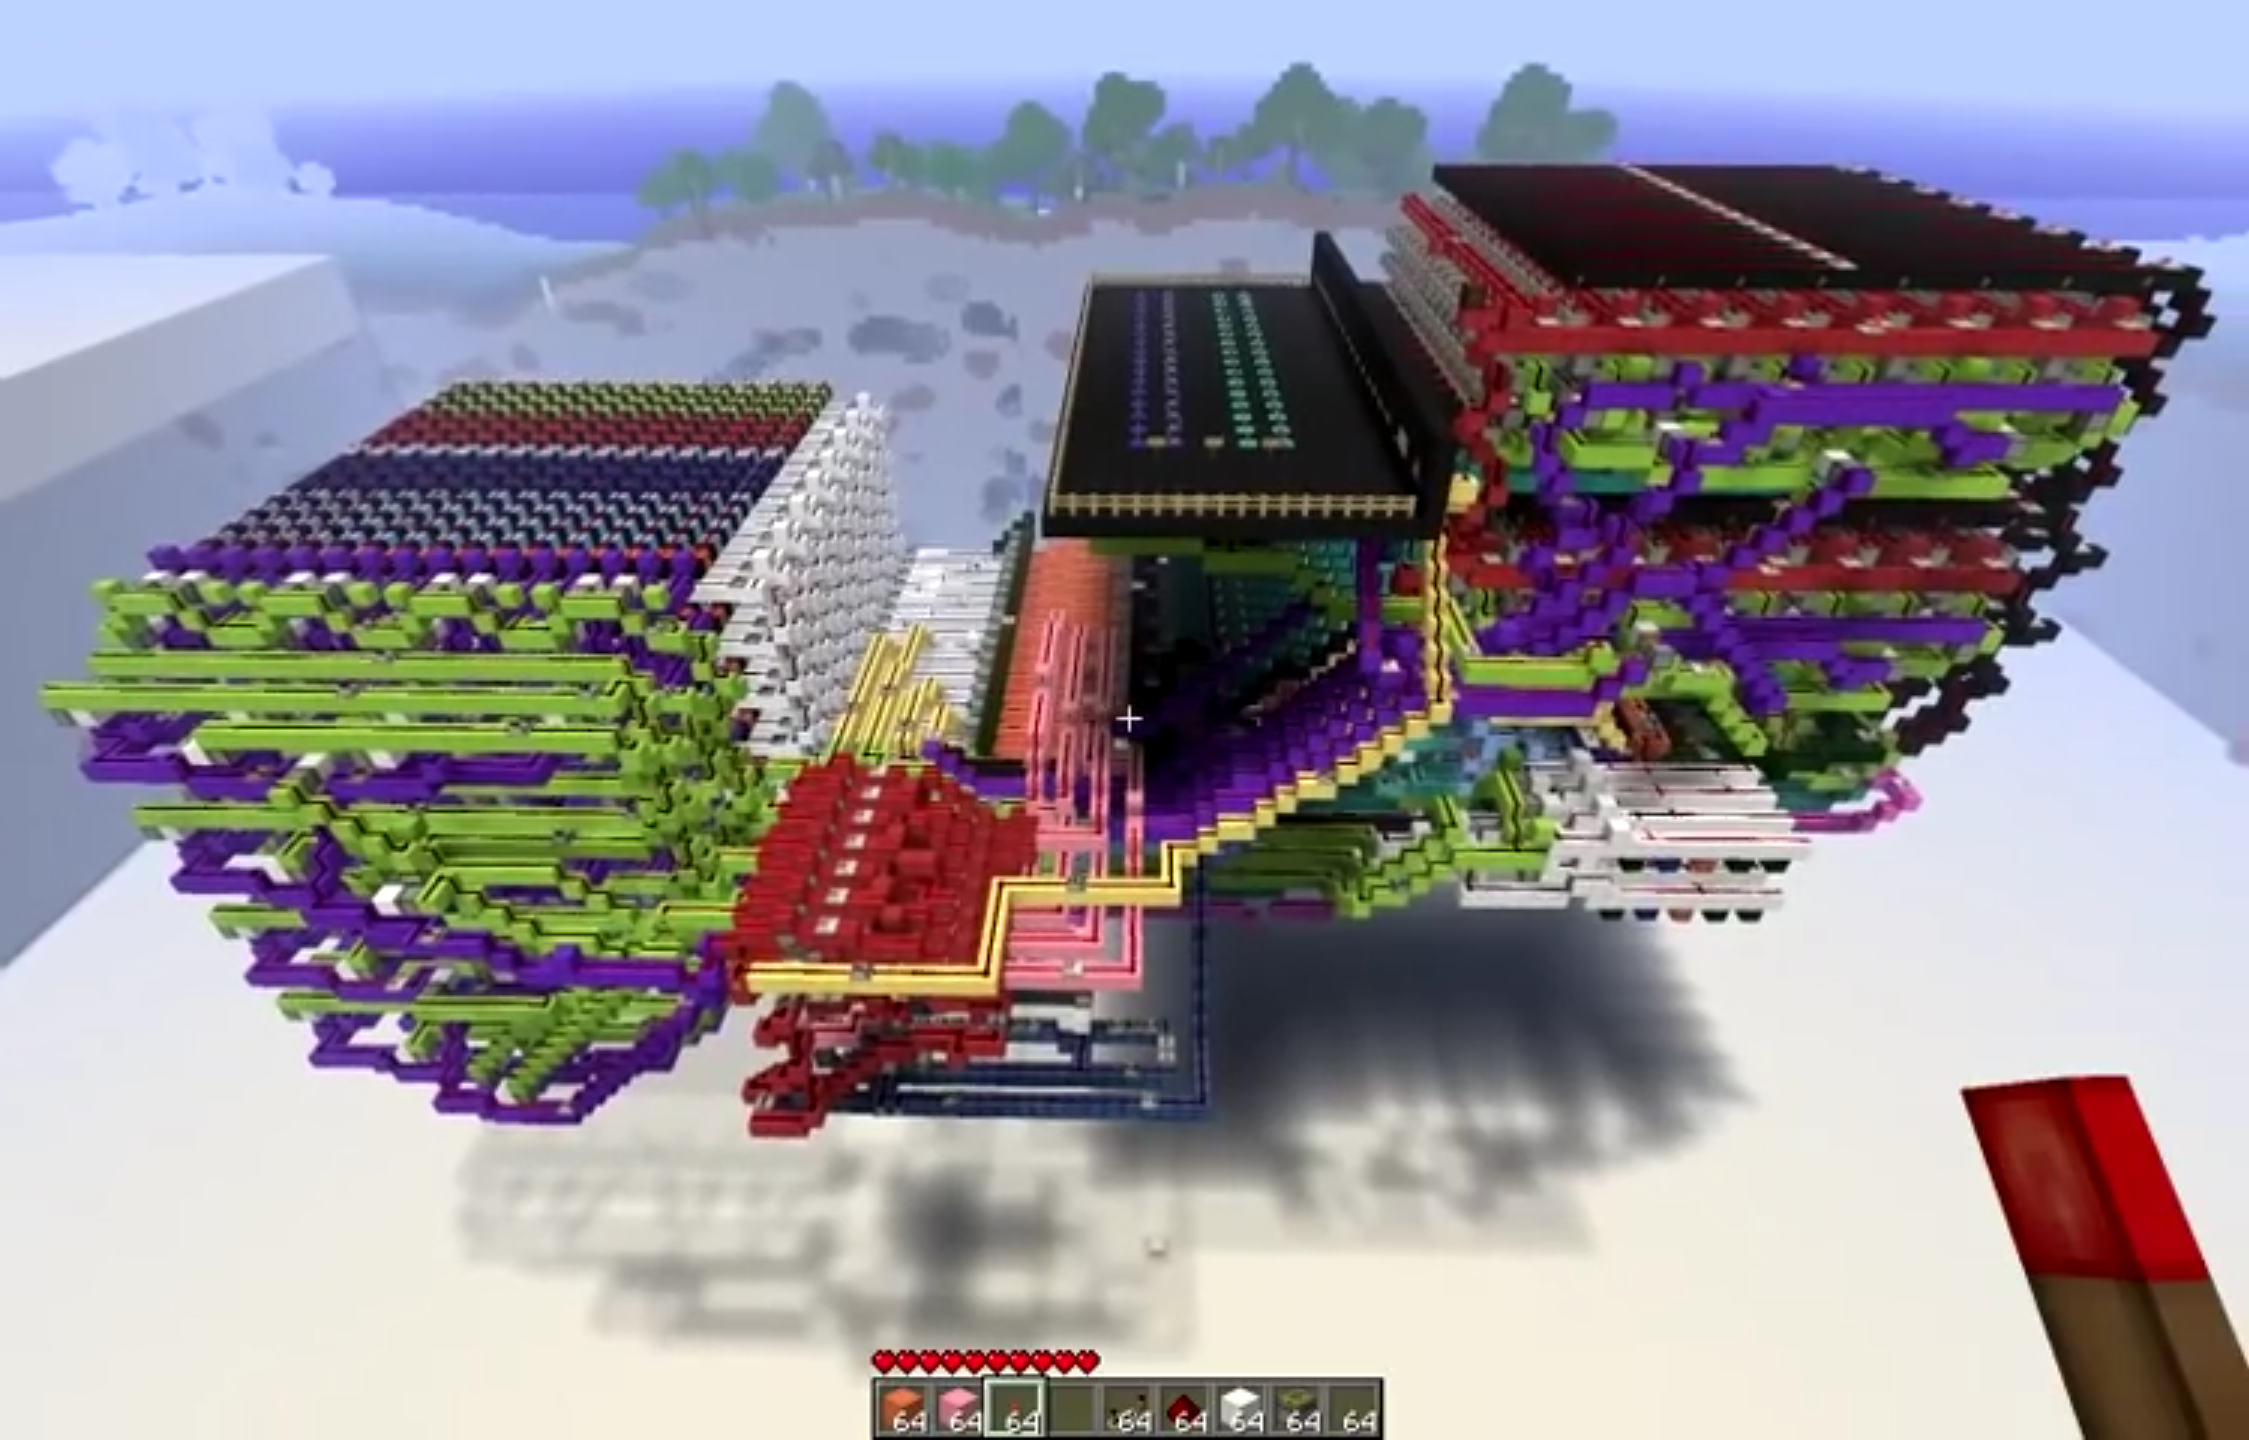
\includegraphics[width=\linewidth]{minecraft.png}
  \caption{Screenshot of a 16 bit computer built in Minecraft by user Ohm.  Full video available on \href{https://www.youtube.com/watch?v=KzrFzkb3A4o}{YouTube}.}
  \label{fig:minecraft}
\end{figure}
The most widely adopted example of discrete design is \href{https://minecraft.net/}{Minecraft}, a PC game that gives players the ability to construct their own worlds from over 100 different block types (Fig \ref{fig:minecraft}).  A subset of these block types form the basis of digital logic in the game and another set of part provide a means of mechanical actuation.  Gameplay and available block types are extendable through various mods and user scripts.
\\

\begin{figure}
  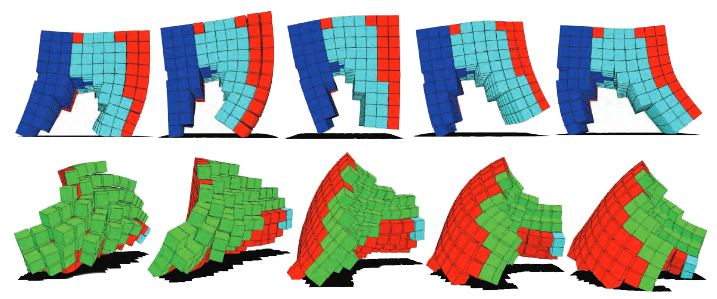
\includegraphics[width=\linewidth]{voxcadWalkers.png}
  \caption{Example gaits of two locomotion robots built from four material types in VoxCAD\cite{Cheney2013b}.}
  \label{fig:voxcadWalkers}
\end{figure}
\href{http://www.voxcad.com/}{Voxcad} is a physics-based design and dynamic simulation environment by Jonathan Hiller where a user designs virtual soft robots from four block types - two active and two passive\cite{Hiller2014a}.  Though the passive block types descended from a simulation of multimaterial 3D printed voxels, the active block types are not easily fabricated and actuated\cite{Hiller2012} and have not been rigorously evaluated.  Interesting work into the optimization of locomotion systems in this virtual design space have been explored (Fig: \ref{fig:voxcadWalkers})\cite{Cheney2013b}\cite{Cheney2013}\cite{Cheney2015}.
\\


\href{http://golly.sourceforge.net/}{Golly} is a 2D cellular automata simulator originally intended for Conway's game of life, but is extendable to other rulesets.  It implements Gosper's "hashlife" algorithm for optimizing the performance of the simulation\cite{Gosper1984}.  In 2010 Andrew Wade published \href{https://www.youtube.com/watch?v=A8B5MbHPlH0}{Gemini}, a self replicating machine designed in Golly using Conway's ruleset.
\\

\begin{figure}
  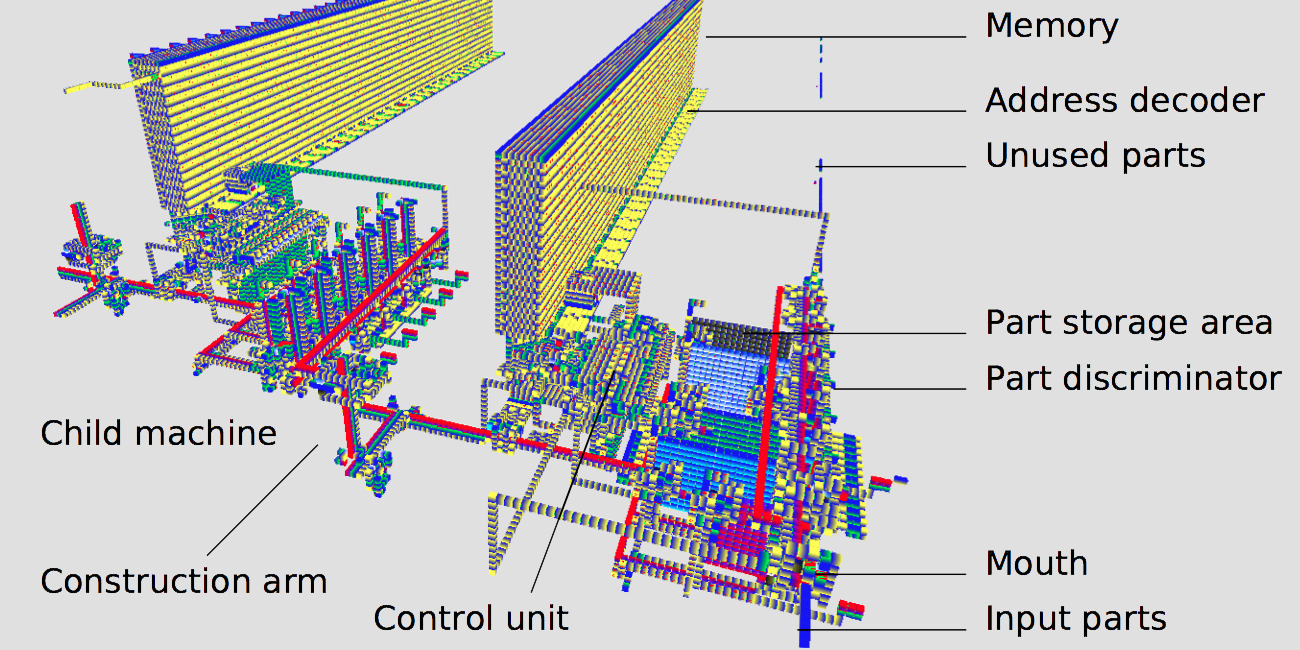
\includegraphics[width=\linewidth]{stevensConstructor.png}
  \caption{A programmable, universal constructor (shown replicating itself) built in CBlock3D by William Stevens from 5040 cells of 6 different types\cite{Stevens2009b}.  Full video of assembly process on  \href{https://www.youtube.com/watch?v=PBXO_6Jn1fs}{YouTube}.}
  \label{fig:stevensConstructor}
\end{figure}
\href{https://www.youtube.com/watch?feature=player_embedded&v=PBXO_6Jn1fs}{CBlock3D} is a 3D cellular automata environment governed by logical and kinematic rules developed by William Stevens\cite{Stevens2007}\cite{Stevens2009}.  It also implements a version of hashlife optimization\cite{Stevens2010}, and Stevens was able to construct and simulate a self-replicating machine within this design environment from 5040 cells of 6 distinct types (Fig: \ref{fig:stevensConstructor})\cite{Stevens2009b}.
\\

\begin{figure}
  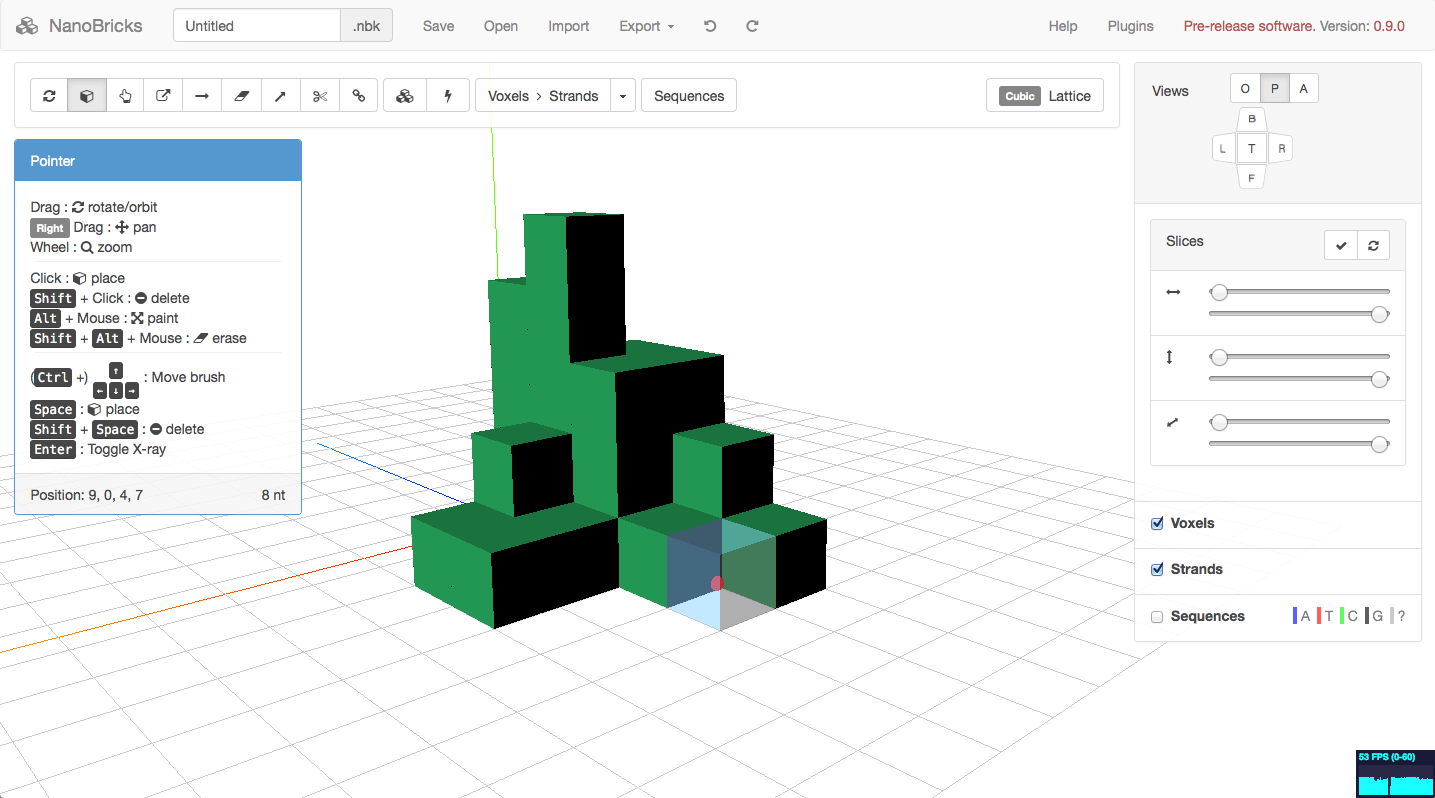
\includegraphics[width=\linewidth]{nanoBricks.png}
  \caption{Screenshot of NanoBricks, a voxel-based design tool for DNA Bricks by the Peng Yin Lab.}
  \label{fig:nanoBricks}
\end{figure}
\href{http://yin.hms.harvard.edu/bricks/try/}{Nanobricks} is a voxel-based design tool for DNA Bricks.  Nanobricks allows a user to design nano-scale structures with voxels on a cubic lattice, and voxel-based designs are converted to sequences and exported as a text file.  Nano bricks does not implement any simulation deformable DNA structures, though others have explored some structural models of DNA with programmable bending\cite{Dietz2009}\cite{Kim2012}.
\\

\begin{figure}
  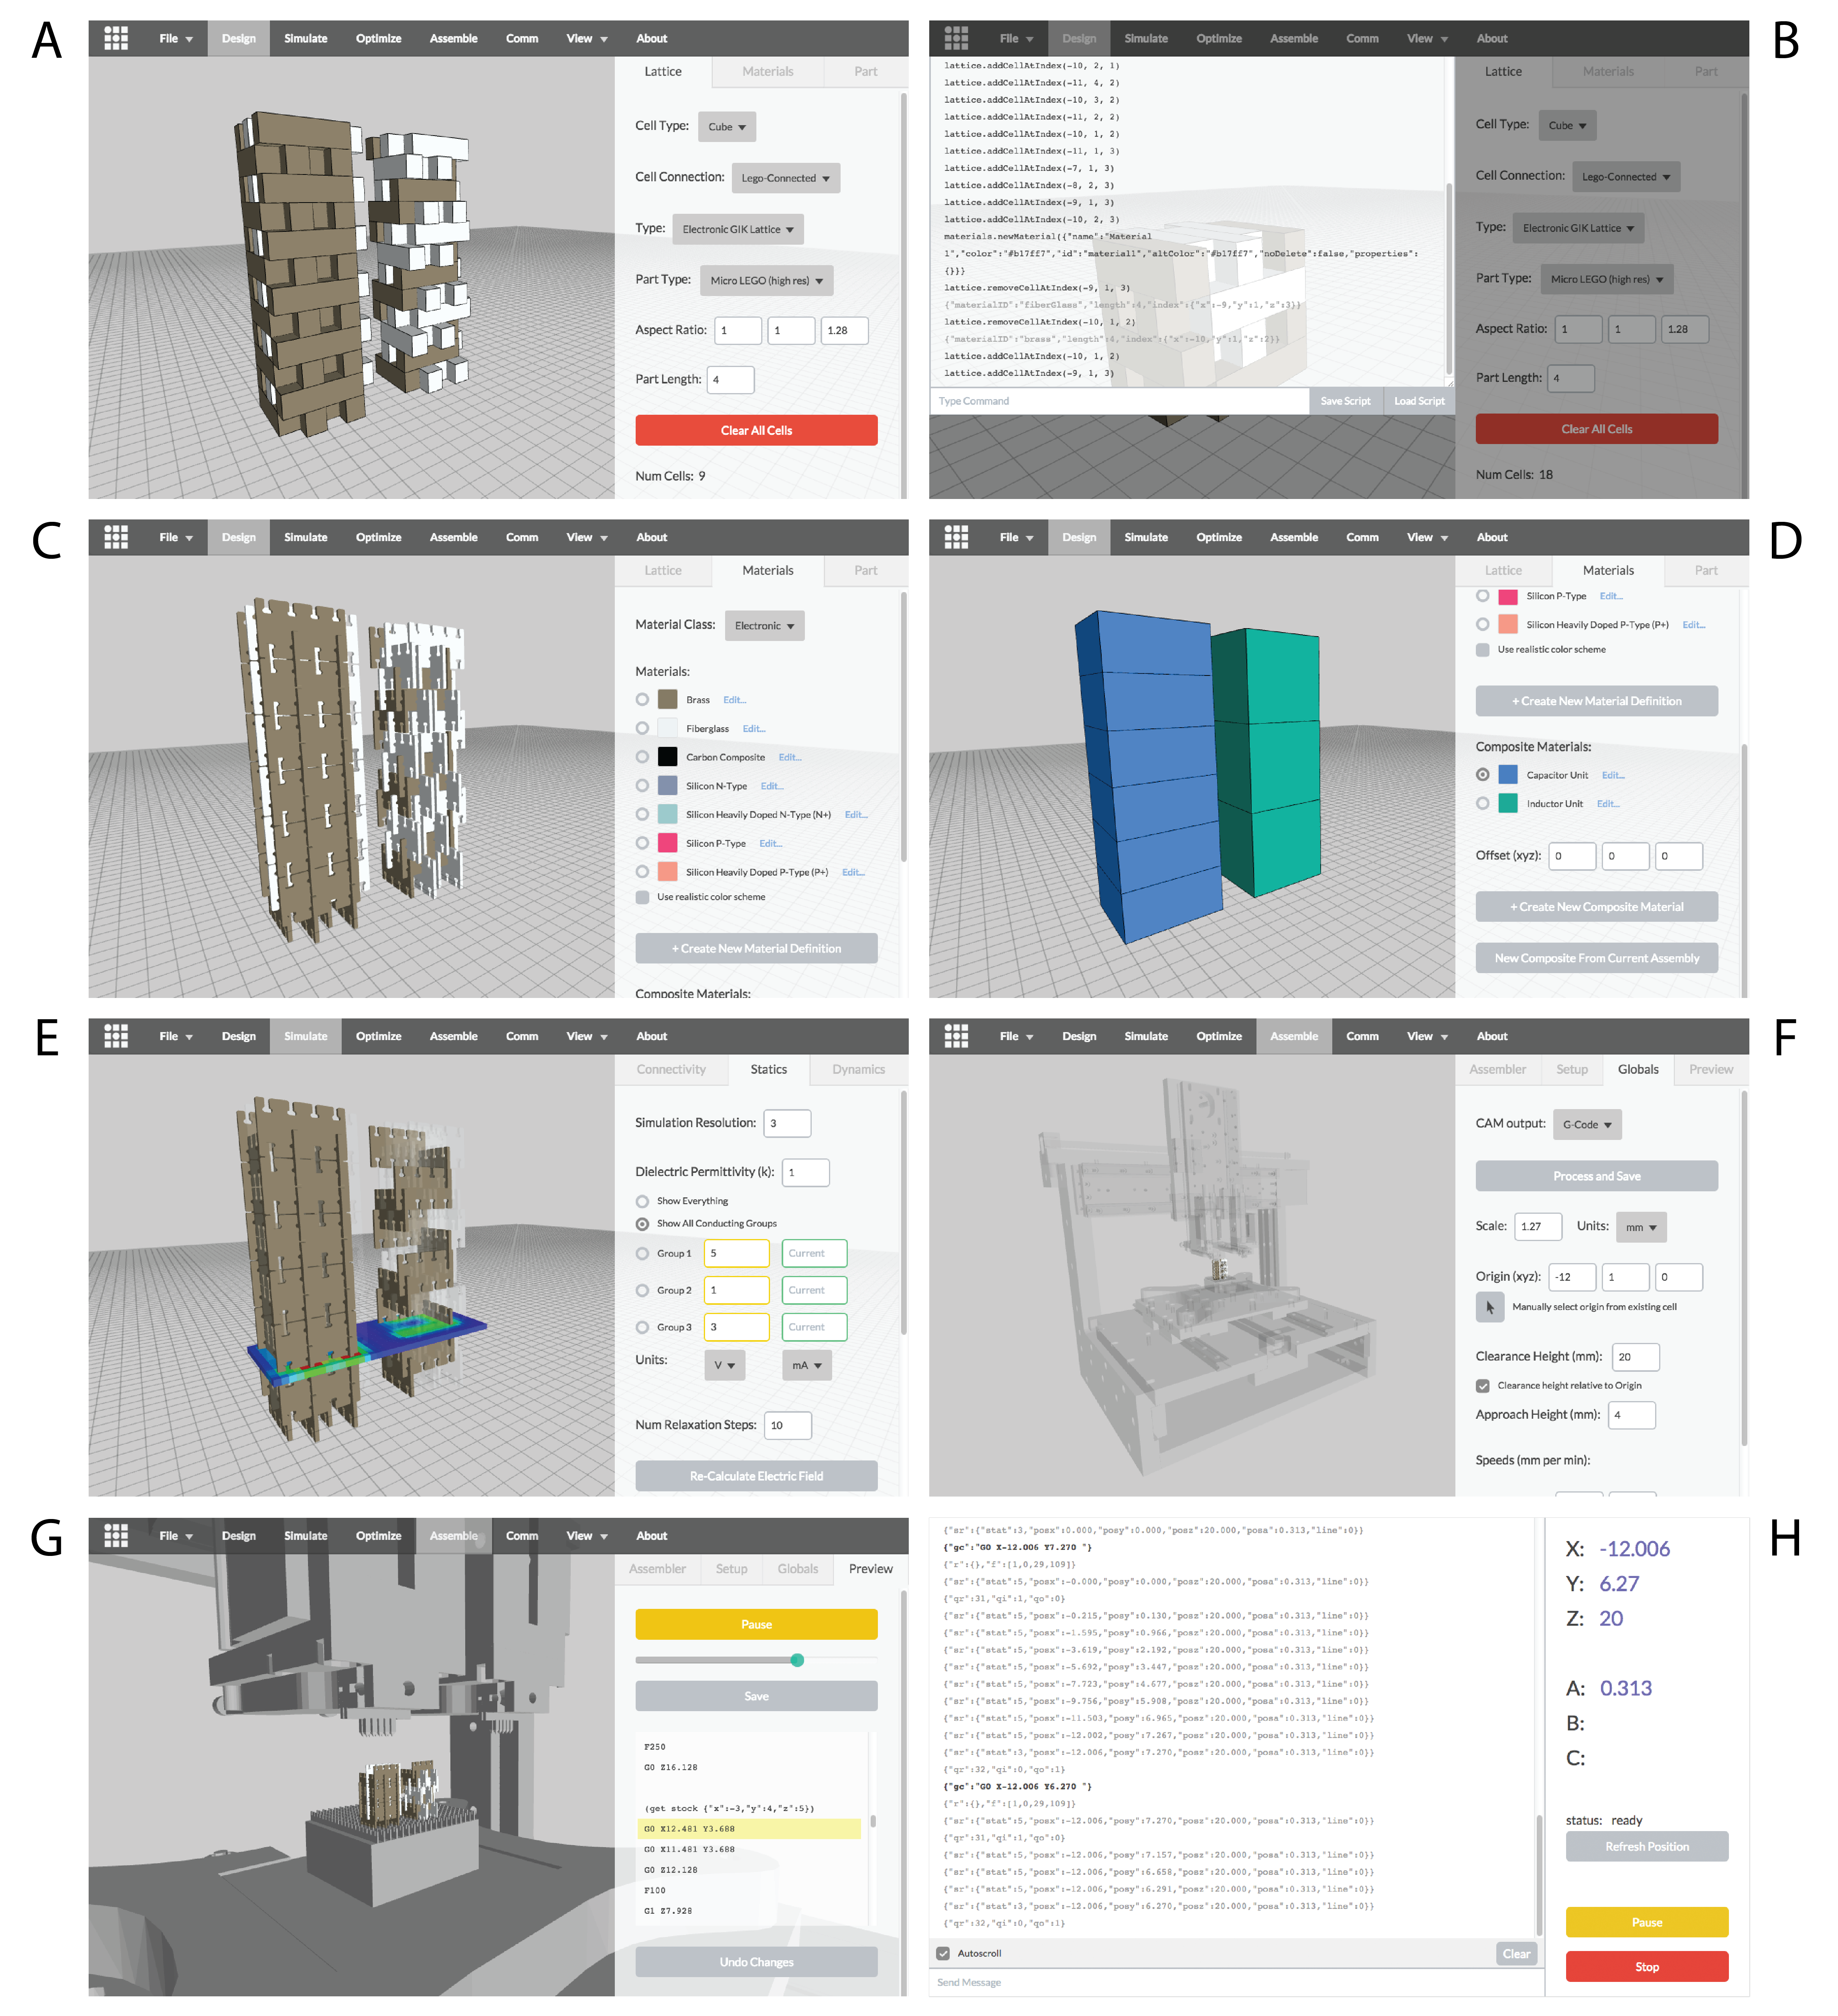
\includegraphics[width=\linewidth]{20151215DMDesignscreenshotsx8.png}
  \caption{Screenshots of my current work with DMDesign, a CAD/Simulation/CAM software package for Digital Materials. Structures are designed from multiple materials in a hierarchical \textbf{(D)}, 3D CAD interface or scripting API \textbf{(B)} that can toggle between a geometric and parts design representation \textbf{(A, C)}. Simulation of the potential field around conducting elements of an LC structure designed from conductive and insulating parts \textbf{(E)}. Path planning and visualization of the assembly process \textbf{(F, G)} and serial interface with machine \textbf{(H)}.}
  \label{fig: designAssemblyGUIWide}
\end{figure}
\href{http://dma.cba.mit.edu/dmdesign/}{DMDesign} is a CAD/CAM environment for digital materials I've been developing that supports the research efforts into part and assembler design at CBA (Fig \ref{fig: designAssemblyGUIWide}).  In DMDesign, users design structures in a virtual 3D environment from many material types, plan out the assembly of a design by a robotic assembler, and communicate in realtime with hardware to physically realize the design.  By abstracting the geometry of the lattice from its decomposition into parts and implementing many lattice types in the CAD workflow, users can design structures ranging from nano to meter scale for a variety of application spaces.

}
